% Present study and efforts, Mechanism Space Explorer.
% Build: tectonic main.tex   (figures: scripts/report/report_figures.py)
% Pending results: search for EVAL.
\documentclass[11pt]{article}

\usepackage[letterpaper,margin=1in]{geometry}
\usepackage[T1]{fontenc}
\usepackage{newtxtext,newtxmath}
\usepackage{microtype}
\usepackage{graphicx}
\usepackage{booktabs}
\usepackage{array}
\usepackage{tabularx}
\usepackage{xcolor}
\usepackage{tikz}
\usetikzlibrary{arrows.meta,positioning}
\usepackage[font=small,labelfont=bf,labelsep=period]{caption}
\usepackage{enumitem}
\usepackage[section]{placeins}
\usepackage{titlesec}
\usepackage[colorlinks=true,linkcolor=black,citecolor=black,
            urlcolor=blue!50!black]{hyperref}

\titleformat{\section}{\normalsize\bfseries}{\thesection}{0.6em}{}
\titleformat{\subsection}{\normalsize\itshape}{\thesubsection}{0.6em}{}
\titlespacing*{\section}{0pt}{2.0ex plus 0.5ex}{0.7ex}
\titlespacing*{\subsection}{0pt}{1.4ex plus 0.3ex}{0.5ex}

\definecolor{ink2}{HTML}{52514E}
\definecolor{muted}{HTML}{898781}
\newcommand{\tba}[1][pending]{\textcolor{muted}{\emph{#1}}}
\newcommand{\kcal}{kcal/mol}
\setlist{itemsep=2pt,topsep=4pt}
\renewcommand{\arraystretch}{1.15}
\setlength{\emergencystretch}{2em}

\title{\vspace{-1.6cm}Would Swapping DFT for a Machine-Learned Potential
Change What a Nanoreactor Finds?\\[4pt]
\large Mechanism Space Explorer: present study and efforts}
\author{Ujjawal Modanwal}
\date{25 November 2026}

\begin{document}
\maketitle

\begin{abstract}
\noindent Nanoreactor simulations have helped to find chemical reactions
without a prior guess. Each step has then needed an accurate energy.
Density functional theory (DFT) has been the usual source of these
energies, but it has been slow. Machine-learned potentials have promised
similar energies in a small fraction of the time. However, it has remained
unclear whether such a swap might change the products, or the paths to
them. In the present study, I have tried to test this on four small
reacting systems. I have found the reactions once with fast xTB
metadynamics and have frozen them. I have then given the same reactions to
five energy models. I have checked every structure they have found with
DFT single points. In my runs, the models have disagreed on single steps.
xTB has placed every CO-forming reaction 39 to 46~\kcal{} too high against
DFT. It has also reversed the order of the two formic acid channels. DFT
on xTB's own shapes has given the reported order. The two models that have
learned from OMol25 have stayed within 0.3 to 2.6~\kcal{} of DFT on
average. However, OMol25 has used this same DFT level, so this has not
been an independent test. The same input has already given different
networks. I have not yet compared whole networks by their products.
Future efforts are being made to implement
better strategies for sampling, detection, refinement and evaluation.
\end{abstract}

% ---------------------------------------------------------------------
\section{Why this study}

Nanoreactor studies have mapped chemistry without a prior guess
\cite{wang2014,grimme2019,zhang2023}. In my runs, I have pushed a box of
molecules hard and have recorded every bond that has broken or formed.
Each molecule and each transition state has then needed an energy. I have
used ``transition state'' to mean the highest point on the lowest path
between two sets of molecules. Its height above the start, the barrier,
has decided how fast a step can run. DFT has given these energies well,
but it has cost minutes to hours per structure. A full DFT pass over my
four systems would have taken about five weeks on my machine.

Machine-learned potentials have learned DFT energies from large data sets.
They have then predicted new energies in milliseconds to seconds. Recent
models that have learned from the OMol25 set have come close to DFT on
test sets \cite{omol25,uma,mace}. They have also sped up transition-state
searches \cite{marks2026}. A nanoreactor study might, therefore, be
shortened from weeks to hours.

However, a good test-set score has not settled this. A nanoreactor has
reported products and the paths that have led to them, not single
energies. Small errors in two competing barriers could flip which path
would win. Errors could also add up along a path. So a model might score
well on single steps and still change the answer. I have wanted to test
the answer itself. My motive has been practical. I have wanted to know
when a machine-learned potential can be trusted for this kind of study. I
have also wanted to know how accurate it would need to be.

% ---------------------------------------------------------------------
\section{The question}

\begin{center}
\fbox{\parbox{0.88\linewidth}{\centering\textbf{Would swapping DFT for a
machine-learned potential change the products, or the paths to them,
predicted by a nanoreactor?}}}
\end{center}

\noindent I have set seven goals for this question. Two goals have built
the data, and one has judged single steps. Three have judged whole
networks, and the last one has compared the cost. Table~\ref{tab:goals}
in Section~\ref{sec:close} has listed how far I have come with each.

% ---------------------------------------------------------------------
\section{Approach}

I have separated finding reactions from judging them. The finding step has
been random and costly, so I have run it only once, with GFN2-xTB
metadynamics \cite{gfn2,grimme2019}. Metadynamics has added a small bias.
This bias has pushed the molecules away from shapes they had already
visited, and it has driven them over barriers within picoseconds. I have
frozen what the runs have found. I have then given the same frozen file to
each energy model. I had thought that one fixed input might give a fairer
test. Any change in the network could then come only from the model
(Figure~\ref{fig:pipeline}).

\begin{figure}[htbp]
\centering
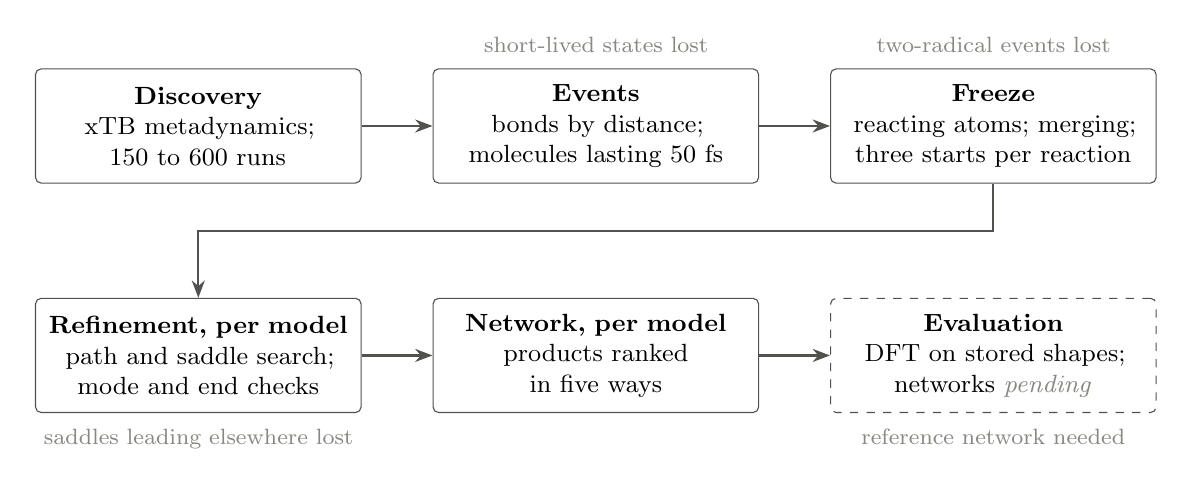
\begin{tikzpicture}[
  box/.style={draw=ink2, rounded corners=2pt, align=center,
    text width=3.9cm, minimum height=1.45cm, font=\small, fill=white},
  todo/.style={box, dashed},
  note/.style={font=\footnotesize, text=muted, align=center,
    text width=4.1cm},
  arrow/.style={-{Stealth[length=2.2mm]}, draw=ink2, thick},
  node distance=0.75cm and 0.9cm]
\node[box] (md) {\textbf{Discovery}\\xTB metadynamics;\\150 to 600
  runs};
\node[box, right=of md] (ev) {\textbf{Events}\\bonds by distance;\\
  molecules lasting 50~fs};
\node[box, right=of ev] (fr) {\textbf{Freeze}\\reacting atoms; merging;\\
  three starts per reaction};
\node[box, below=1.45cm of md] (rf) {\textbf{Refinement, per model}\\path
  and saddle search;\\mode and end checks};
\node[box, right=of rf] (nw) {\textbf{Network, per model}\\products
  ranked\\in five ways};
\node[todo, right=of nw] (evl) {\textbf{Evaluation}\\DFT on stored
  shapes;\\networks \tba};
\node[note, above=0.08cm of ev] {short-lived states lost};
\node[note, above=0.08cm of fr] {two-radical events lost};
\node[note, below=0.08cm of rf] {saddles leading elsewhere lost};
\node[note, below=0.08cm of evl] {reference network needed};
\draw[arrow] (md) -- (ev);
\draw[arrow] (ev) -- (fr);
\draw[arrow] (fr.south) -- ++(0,-0.6) -| (rf.north);
\draw[arrow] (rf) -- (nw);
\draw[arrow] (nw) -- (evl);
\end{tikzpicture}
\caption{The pipeline of the present study. Solid boxes: the steps I have
run. Dashed box: the evaluation I have only partly run. Gray notes: where each
step has lost reactions (Section~\ref{sec:limits}).}
\label{fig:pipeline}
\end{figure}

I have chosen four small systems with known chemistry
(Table~\ref{tab:systems}). Each one has tested a different kind of
choice. Formic acid has offered two competing channels. Formic acid with
water has added a helper water. Formaldehyde with ammonia has offered a
two-step path. Cyclopentadiene with maleic anhydride has offered the endo
and exo Diels--Alder adducts. Each system has had a literature result to
check against.

\begin{table}[htbp]
\centering
\caption{The four systems. MD runs: the metadynamics runs behind each
frozen set. I have added one reaction by hand to HCHO + NH$_3$ and one to
CPD + MA. The MD had missed both.}
\label{tab:systems}
\small
\begin{tabular}{@{}llrrrl@{}}
\toprule
System & Start & Atoms & MD runs & Reactions & Reported at \\
\midrule
HCOOH & formic acid, trans and cis & 5 & 600 & 4 & 1000 K \\
HCOOH + H$_2$O & formic acid and water & 8 & 600 & 10 & 1000 K \\
HCHO + NH$_3$ & formaldehyde and ammonia & 8 & 600 & 13 & 298, 600 K \\
CPD + MA & cyclopentadiene and maleic anhydride & 20 & 150 & 38 &
298, 493 K \\
\bottomrule
\end{tabular}
\end{table}

I have compared five energy models (Table~\ref{tab:engines}). GFN2-xTB has
served as the fast, semi-empirical baseline. UMA and MACE-OMol25 have
learned from OMol25 at the $\omega$B97M-V/def2-TZVPD level
\cite{omol25,uma,mace}. AIMNet2-NSE has learned from $\omega$B97M data
and has handled spin \cite{aimnet2}. ANI-1xnr has learned from nanoreactor
data at the BLYP level \cite{ani1xnr,torchani}. A full DFT search has
cost too much on my machine (Table~\ref{tab:cost}). So I have used DFT at
the OMol25 level only for single points on each model's structures
\cite{wb97mv,orca}. I have reported each system at
the temperature of its literature source, and at a higher one where I have
had it.

\begin{table}[htbp]
\centering
\caption{The energy models. The figures have coloured each model by its
family (blue, orange, aqua) and have given each model its own marker.}
\label{tab:engines}
\small
\begin{tabular}{@{}lllll@{}}
\toprule
Model & Family (colour) & Training data & Spin & Version \\
\midrule
GFN2-xTB & semi-empirical (blue) & fitted method & yes &
tblite 0.8.0; xtb 6.7.1 \\
UMA & OMol25 (orange) & OMol25 and other sets & yes & uma-s-1p2p1 \\
MACE-OMol25 & OMol25 (orange) & OMol25 & yes & extra large \\
AIMNet2-NSE & other ML (aqua) & $\omega$B97M data & yes &
aimnet2-nse\_0 \\
ANI-1xnr & other ML (aqua) & nanoreactor data, BLYP & no &
torchani 2.12 \\
DFT check & --- & --- & yes & ORCA 6.1.1, single points \\
\bottomrule
\end{tabular}
\end{table}

% ---------------------------------------------------------------------
\section{What I have run}

\paragraph{Discovery.} I have run metadynamics with xtb 6.7.1 inside a
soft spherical wall. I have used a 300~K bath, a 0.5~fs step, and a saved
frame every 5~fs. Each run has lasted 10~ps. Each one has started from a
frame of a 100~ps run without bias. I have taken the settings from Zhang
et al.~\cite{zhang2023} and Grimme~\cite{grimme2019}, and then I have
scanned the push strength. For each small system, I have used 600 runs:
two push strengths and six groups of 50. For CPD + MA, I have used 150
runs at three gentler pushes. Independent check runs have found the main
channels again. For example, the main and check groups have given 44 and
24 decarboxylation events.

\paragraph{Events and freeze.} I have read bonds from distances. Two atoms
have counted as bonded when they have sat closer than 1.2 times the sum of
their covalent radii. A molecule has counted only if it has lasted 50~fs.
An event has meant a change between two such sets of molecules. Freeze has
then kept only the atoms whose bonds have changed. It has rejected events
with two or more radicals on one side. I had left open-shell singlets and
triplets out of scope. It has relaxed both sides with xTB. It
has rejected events whose molecules have changed on relaxing. It has
merged events with the same reacting molecules, stereo included, and has
kept the first three as starting points (Figure~\ref{fig:discovery}). In
the three small systems, most events have carried two radicals, so freeze
has dropped them.

\begin{figure}[htbp]
\centering
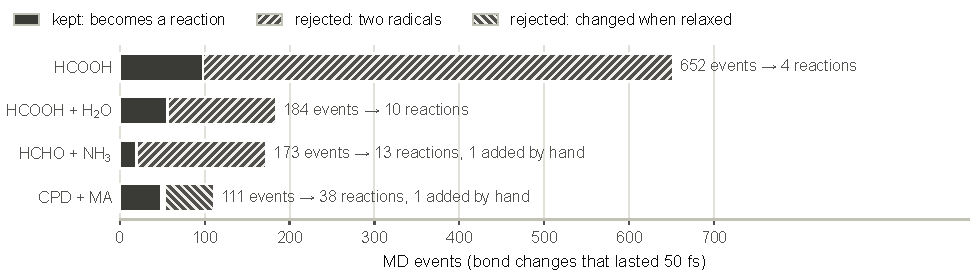
\includegraphics[width=\linewidth]{figures/fig2_discovery.pdf}
\caption{MD events kept and rejected by freeze, per system. Dark: events
that have become reactions. Hatched: events that freeze has rejected. For
CPD + MA, the per-reaction event counts have added up to 56. The freeze
statistics have given seven fewer; I have not yet traced this gap.}
\label{fig:discovery}
\end{figure}

\paragraph{Refinement.} For each model, I have first optimized every
molecule and have computed its vibrations. I have then searched each
reaction from each of its starting points. Each search has built a path of
13 images between the two relaxed ends. It has refined the highest image
to a saddle with Sella~\cite{sella} and has checked the vibrations. I have
accepted a saddle only when it has had exactly one imaginary mode below
$-50$~cm$^{-1}$. I have then pushed the saddle a little along that mode
and have minimized the energy. Both sides have had to reach the expected
molecules. The ML models have also tried xTB's saddle as a start. I have kept
the confirmed saddle with the lowest free energy. I have measured each
barrier from the separated reacting molecules, at 1~atm. Before computing
free energies, I have raised every real vibration below 100~cm$^{-1}$ to
100~cm$^{-1}$~\cite{truhlar2011}.

\paragraph{DFT check.} I have then computed one DFT energy for every
stored saddle and molecule of every model. I have used
$\omega$B97M-V/def2-TZVPD in ORCA 6.1.1, the level of OMol25
\cite{wb97mv,orca}. That has made 467 jobs: 110 saddles and 357
molecules. On each saddle, I have also computed the DFT force. I have not
optimized anything with DFT. So each DFT barrier has stood on the model's
own shapes. A large DFT force on a saddle has meant that DFT would have
moved it far. For free energies, I have added each model's own vibrational
correction to the DFT energy. Six molecules have kept an imaginary mode
after their model's refinement, so I have left them out.

\paragraph{Paths.} I have also followed the intrinsic reaction coordinate
(the steepest path down from a saddle, on both sides) on each model
\cite{fukui1981,sella}. I have done this for every saddle of the three
small systems, and for each model's two Diels--Alder saddles: 80 paths. On
21 paths, Sella's IRC has stalled, and I have let it carry on past the
stall. Such a path has stayed continuous, but it has not been an exact
IRC. I have then computed 1,281 DFT energies along these paths. The
highest DFT point on a path between the two valleys has given an upper
limit to the DFT saddle energy. This has assumed that both ends have
sat in the DFT valleys of the same molecules.

\paragraph{Cost.} Table~\ref{tab:cost} has listed what each model has
cost. I have run everything on a 10-core laptop, except MACE-OMol25, which
I have moved to a free T4 GPU. The free GPU time has run out before the
last five CPD + MA reactions. I have run those five on the laptop, in
3.4~h.

\begin{table}[htbp]
\centering
\caption{What each model has cost. One energy and force: 20 atoms,
one idle laptop core; DFT on four cores.}
\label{tab:cost}
\small
\begin{tabularx}{\linewidth}{@{}l>{\raggedright\arraybackslash}X
>{\raggedright\arraybackslash}X@{}}
\toprule
Model & One energy and force & Refinement \\
\midrule
GFN2-xTB & 3.3 ms (laptop) & 2 min or less per small system; 3.4 h for
CPD + MA \\
ANI-1xnr & 4.1 ms (laptop) & 3 to 32 min per system \\
AIMNet2-NSE & 4.3 ms (laptop) & 1.3 h for CPD + MA \\
UMA & 38 ms (laptop) & 5.1 h for CPD + MA \\
MACE-OMol25 & 222 ms laptop; 268 ms T4; 129 ms T4 with faster GPU
code & 3.2 to 9.7 h per small system (T4); CPD + MA: 11.5 h on two T4s,
then 3.4 h on the laptop \\
DFT & 3.6 to 4.5 min (4 cores) & vibrations alone: 7 to 9 h per
structure; the single-point check: about 16 h \\
\bottomrule
\end{tabularx}
\end{table}

% ---------------------------------------------------------------------
\section{What I have found}

\subsection{Confirmed transition states}

Figure~\ref{fig:outcomes} has shown how each search has ended. On formic
acid, every model except ANI-1xnr has confirmed all four saddles. ANI-1xnr
has taken no spin, so it has skipped the two radical steps. Coverage has
fallen as the systems have grown. On CPD + MA, the models have confirmed
only 4 to 11 of 38 reactions. About half of these reactions have ended in
a search that has broken down. About a fifth have ended with a saddle that
has led to other molecules. The models have failed on different
reactions. So a fair network comparison is expected to need two views:
each model's own reactions, and the reactions every model has shared.

\begin{figure}[htbp]
\centering
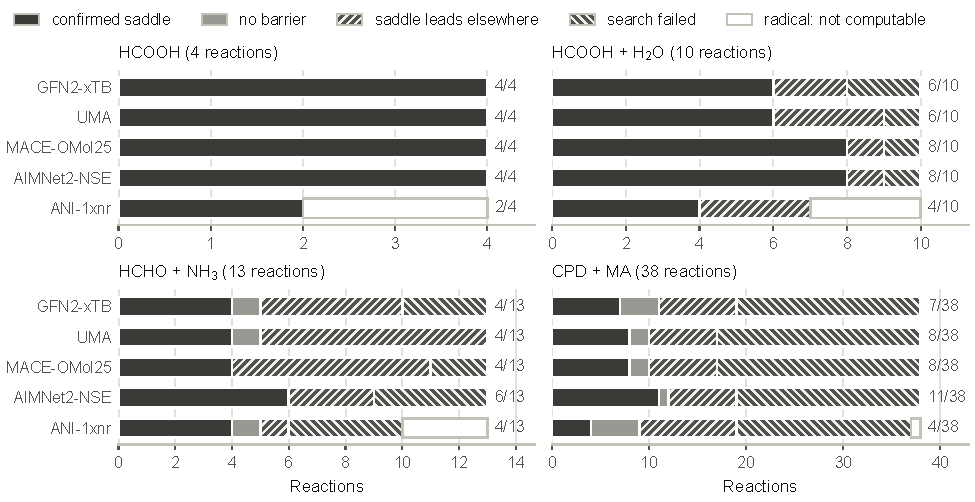
\includegraphics[width=\linewidth]{figures/fig3_outcomes.pdf}
\caption{How each model's transition-state searches have ended. Each bar:
all frozen reactions of one system. Number at right: confirmed saddles
over all reactions. Hatched: lost reactions, where the search has found a
saddle that has led to other molecules, or has broken down.}
\label{fig:outcomes}
\end{figure}

\subsection{The networks each model has kept}

Figure~\ref{fig:networks} has drawn two of the frozen networks. Each
circle has stood for one state of the whole box, and each arrow for one
reaction. The five squares on an arrow have marked the models that have
kept it. In HCOOH + H$_2$O, every model has kept the bare decarboxylation
and dehydration. Every model has also kept the addition of water to
HC(OH)$_3$ and the breakup of carbonic acid. The water-assisted versions
have survived only for MACE-OMol25, and for AIMNet2-NSE in dehydration. In
HCHO + NH$_3$, every model has kept three steps. These steps have been the
addition to aminomethanol, its dehydration, and the split of HCHO into CO
and H$_2$. None of the other six
steps from the start has survived in more than two models. Three of them
have survived in none. The radical chains have sat apart from the start.
This has happened because freeze has removed the two-radical steps that
would have joined them. So the models have already built different
networks from the same input.

\begin{figure}[htbp]
\centering
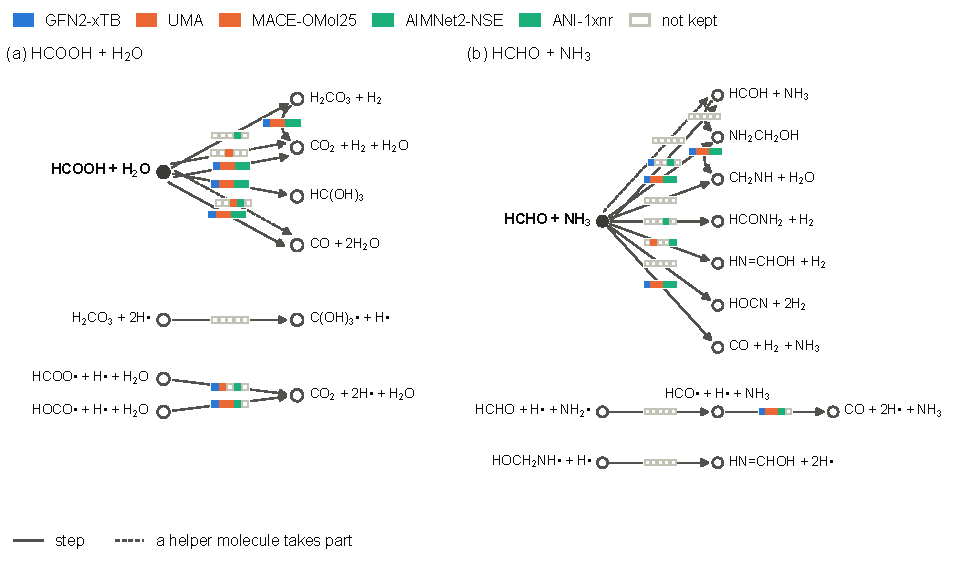
\includegraphics[width=\linewidth]{figures/fig_networks.pdf}
\caption{Two of the frozen networks, with each model's verdict. Circles:
states of the whole box; filled circle: the start. Arrows: reactions;
dashed arrows: a helper molecule has taken part. Squares on each arrow,
from left to right: GFN2-xTB, UMA, MACE-OMol25, AIMNet2-NSE and ANI-1xnr.
A filled square: the model has kept the step. Such a step has had a
confirmed saddle or no barrier, and every molecule has been a true minimum.
The radical chains at the bottom have sat apart. Freeze has dropped the
two-radical steps that would have joined them to the start.}
\label{fig:networks}
\end{figure}

\subsection{Steps against DFT}

Figure~\ref{fig:dft} has compared each model with DFT on the model's own
shapes. UMA has stayed within 1~\kcal{} of DFT on 18 of its 22 barriers,
and MACE-OMol25 on 17 of 23. Table~\ref{tab:dft} has listed the mean
errors. However, both models have learned from data at this same DFT
level. So this match has shown that they have kept their training level
on reacting structures. It has not been an independent test. AIMNet2-NSE
has missed by 3.1 to 9.2~\kcal{} on average, and ANI-1xnr by 10.7 to
26.1~\kcal{}. xTB has placed 16 of its 21 barriers too low.

The DFT force on each saddle has shown how far DFT would move it. On the
UMA and MACE-OMol25 saddles, its median has stayed at 0.11 to
0.30~eV/\AA{}. On the other saddles, it has reached 1 to 3~eV/\AA{}. So
for the other three models, I have measured energy errors on shapes that
DFT would not keep.

For reaction energies, xTB has placed every CO-forming reaction 39 to
46~\kcal{} too high. For HCOOH $\to$ CO + H$_2$O, UMA, MACE-OMol25 and
AIMNet2-NSE have stayed within 1.2~\kcal{}. ANI-1xnr has placed it
9.3~\kcal{} too low. A model that has misplaced a product by 40~\kcal{}
might misjudge how much of that product would form.

Two CPD + MA structures have stood apart. In one step, a single C--C bond
has joined the two molecules. DFT has put this adduct 36 to 43~\kcal{}
above the start on four models' shapes. That has been above the DFT
energy of each model's own saddle. So the adduct might not be a DFT
minimum at all. A closed-shell DFT energy might also have overrated it, if
it has carried two radical centres. UMA and MACE-OMol25 have placed it
17.6 and 17.8~\kcal{} below DFT, respectively. xTB and ANI-1xnr have
placed it about 34~\kcal{} below. In another step, DFT has
put ANI-1xnr's saddle 38.9~\kcal{} below its reactant. So that error, of
$+49.0$~\kcal{}, has had no clear meaning. Without it, the CPD + MA mean
for ANI-1xnr has been 1.8~\kcal{}.

\begin{figure}[htbp]
\centering
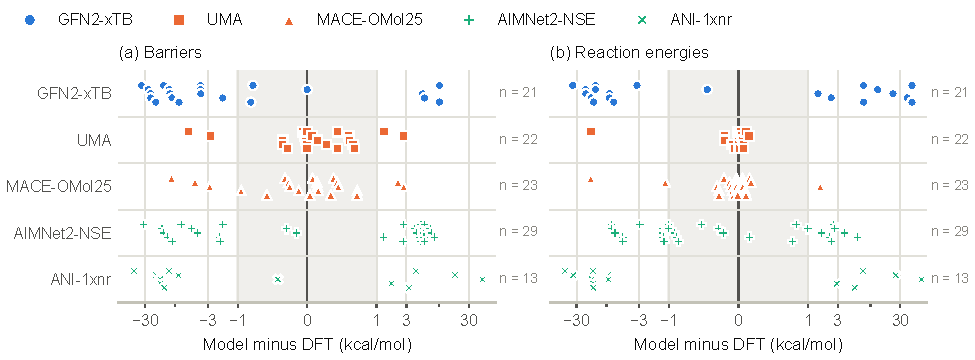
\includegraphics[width=\linewidth]{figures/fig4_dft.pdf}
\caption{Each model against DFT on the model's own shapes. One marker per
saddle (a) or per reaction (b), from all four systems. Barriers: energy
from the separated reacting molecules. Gray band: $\pm1$~\kcal{}. Axis:
linear within $\pm1$~\kcal{}, logarithmic beyond.}
\label{fig:dft}
\end{figure}

\begin{table}[htbp]
\centering
\caption{Mean absolute barrier error against DFT, in \kcal{}, with the
number of saddles in brackets. Last column: the range of the median DFT
force on each model's saddles over the four systems.}
\label{tab:dft}
\small
\begin{tabular}{@{}lrrrrr@{}}
\toprule
Model & HCOOH & HCOOH + H$_2$O & HCHO + NH$_3$ & CPD + MA & DFT force (eV/\AA) \\
\midrule
GFN2-xTB & 9.86 (4) & 8.67 (6) & 16.59 (4) & 11.32 (7) & 0.99--1.97 \\
UMA & 0.35 (4) & 0.25 (6) & 0.43 (4) & 1.67 (8) & 0.11--0.19 \\
MACE-OMol25 & 1.01 (4) & 0.52 (7) & 0.93 (4) & 2.61 (8) & 0.15--0.30 \\
AIMNet2-NSE & 4.83 (4) & 3.07 (8) & 8.02 (6) & 9.21 (11) & 1.19--1.38 \\
ANI-1xnr & 18.79 (2) & 10.69 (4) & 26.09 (3) & 13.59 (4) & 2.17--3.08 \\
\bottomrule
\end{tabular}

\end{table}

\subsection{Barriers}

Figure~\ref{fig:barriers} has collected the barriers. Open markers have
shown DFT on each model's own shapes. UMA and MACE-OMol25 have agreed
within 0.5~\kcal{} on 13 of the 20 saddles they have shared. The largest
gap has been 2.7~\kcal{}. Wherever the gap has exceeded 0.5~\kcal{}, the
two models have still found the same saddle geometry. So the gaps have
come from the energies, not from the search. The two models have used
different designs but have learned from the same data. So the data has
seemed to matter more than the design. AIMNet2-NSE has sat above the mean
of the two OMol25 models on every step in the figure, by 2.2 to
21.5~\kcal{}. ANI-1xnr has departed from them by $-18$ to $+16$~\kcal{},
with no clear pattern. For the addition of NH$_3$ to HCHO, xTB has given
26~\kcal{} and the OMol25 models 39~\kcal{}. DFT on the five models'
shapes has given 37.6 to 39.2~\kcal{}. The literature guides (31 to
34~\kcal{}) have come from other methods \cite{zhang2023,ice2024}. For the
dehydration of aminomethanol, UMA and MACE-OMol25 have landed on the
literature guide of 55.0 to 55.9~\kcal{} \cite{feldmann2005}. DFT on their
shapes has given 55.0~\kcal{} as well. For both Diels--Alder steps, the ML
models have sat 13 to 18~\kcal{} above xTB. DFT on every model's shapes
has given 19.8 to 22.5~\kcal{} for endo and 22.3 to 24.5~\kcal{} for exo.
So xTB's low Diels--Alder barriers have come from its energies.

\begin{figure}[htbp]
\centering
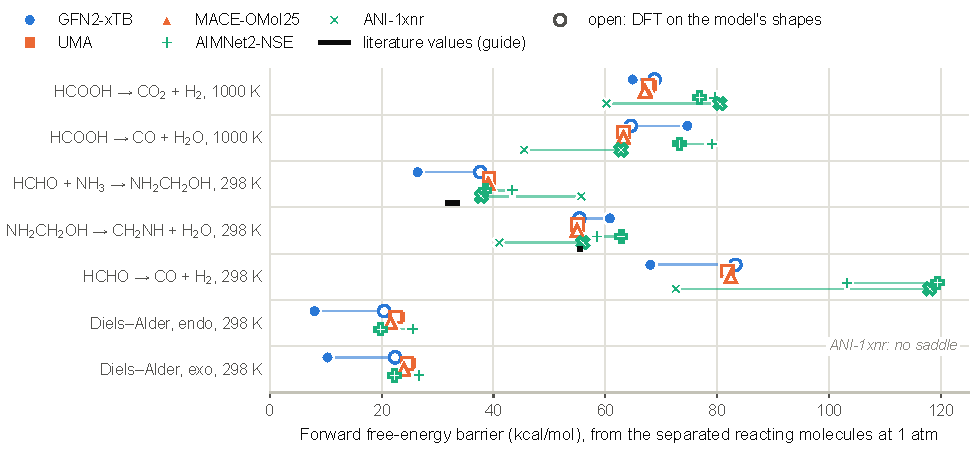
\includegraphics[width=\linewidth]{figures/fig5_barriers.pdf}
\caption{Forward free-energy barriers. Lanes: one per model within each
row. Open markers: the DFT energy on the model's own shapes, plus the
model's own free-energy correction; a thin line joins each pair. Black bars: literature values, as guides only; the sources have used
other methods and might report a different kind of barrier. The other rows
have had no single literature number; Figure~\ref{fig:select} has used
their reported trends instead.}
\label{fig:barriers}
\end{figure}

\subsection{Which channel has won}

The products have depended on which of two competing steps would run
faster. Figure~\ref{fig:select} has shown two such contests. For formic
acid at 1000~K, the literature has reported that dehydration has dominated
in the gas phase. UMA, MACE-OMol25 and ANI-1xnr have agreed. AIMNet2-NSE
has called it a tie. xTB has reversed the order by 9.8~\kcal{}. At
1000~K, that gap would make decarboxylation about 140 times faster. DFT
on each model's shapes has put dehydration first in every case. Its lead
has been 3.6 to 4.4~\kcal{}, and 17.7~\kcal{} on ANI-1xnr's shapes. So
xTB's flip has come from its energies, not from its shapes. For the
Diels--Alder pair, every model that has found both saddles has favoured
endo, by 1.1 to 2.3~\kcal{}. DFT on the same shapes has favoured endo by
1.9 to 2.5~\kcal{}. Both ranges have stayed close to the reported
2.2~\kcal{}. So xTB, the model that has driven my discovery runs,
has already flipped one product preference. This has given a first,
step-level answer to my question.

\begin{figure}[htbp]
\centering
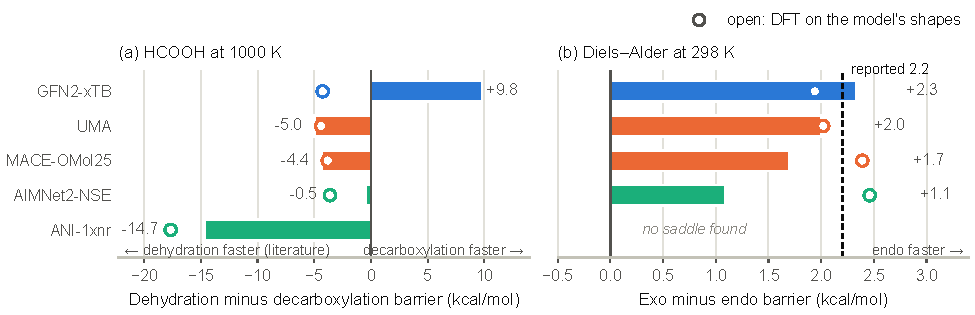
\includegraphics[width=\linewidth]{figures/fig6_selectivity.pdf}
\caption{Which of two competing steps each model has made faster.
(a)~Formic acid at 1000~K: negative values, dehydration faster, as the
literature has reported for the gas phase. (b)~Diels--Alder at 298~K:
positive values, endo faster; dashed line, the reported gap of
2.2~\kcal{}. Open circles: DFT on each model's own shapes.}
\label{fig:select}
\end{figure}

\subsection{Paths from the saddles}

Of the 80 paths, 79 have ended on the molecules of their reaction. The one
exception has been an xTB path in HCHO + NH$_3$, which has run out of
steps on both sides. So my short end check has held on the saddles I have
tested this way. On the UMA and MACE-OMol25 paths, the highest DFT point
has sat on the model's saddle, or within 0.02~\kcal{} of it. One UMA path
has peaked 0.45~\kcal{} higher, and one MACE-OMol25 path 0.09~\kcal{}
higher. So the DFT energy at their saddles has itself been an upper limit.
On xTB paths, the DFT peak has sat up to 2.9~\kcal{} above the saddle. On
AIMNet2-NSE paths, it has sat up to 2.1~\kcal{} above, except on one
formaldehyde step (15.2~\kcal{}). On ANI-1xnr paths, it has sat up to
10.2~\kcal{} above. For the Diels--Alder steps, the MACE-OMol25 paths have
given the lowest limits: 7.4~\kcal{} for endo and 9.5~\kcal{} for exo.
These have been energies, not free energies. Endo has again come out
lower, by 2.1~\kcal{}.

\subsection{Findings in brief}

\begin{itemize}
\item The choice of model has seemed to change the chemistry. xTB has
misplaced CO-forming reactions by about 40~\kcal{} and has flipped the
formic acid channel order. DFT on xTB's own shapes has given the reported
order.
\item The data has seemed to matter more than the design. Two OMol25
models have agreed within 2.7~\kcal{} on every shared saddle, and within
0.5~\kcal{} on 13 of 20. Both have stayed close to DFT, but OMol25 has
used the same DFT level.
\item Selectivity has held better than absolute barriers. All models that
have found both Diels--Alder saddles have favoured endo, but their barriers
have differed by up to 18~\kcal{}.
\item Training on nanoreactor data alone has not helped here. ANI-1xnr has
confirmed the fewest saddles and has scattered the most, against DFT too.
\item The same input has already given different networks
(Figure~\ref{fig:networks}).
\item My own filters have lost many reactions before any model has seen
them (Section~\ref{sec:limits}).
\end{itemize}

% ---------------------------------------------------------------------
\section{Pending comparisons (\tba)}
\label{sec:eval}

% EVAL: fill the comparison table and the yield figure when the rankings
% and the reference network exist.
I have built the code for this part, but I have not yet run it on the
final data. The DFT check has settled the step errors
(Figure~\ref{fig:dft}). A DFT network on the same shapes might now be
built from those single points. Each model's network is
planned to be ranked in five ways. These rankings are expected to range
from a simple free-energy filter to a kinetic simulation of the yields
after one hour. The five comparisons in Table~\ref{tab:eval} are then
planned.

\begin{table}[htbp]
\centering
\caption{The comparisons. I have measured the step errors against DFT.
The product and cost comparisons have needed no reference, so they can be
run now. The other two have needed a reference network.}
\label{tab:eval}
\small
\begin{tabularx}{\linewidth}{@{}l>{\raggedright\arraybackslash}Xll@{}}
\toprule
Comparison & Question & Reference needed & Result \\
\midrule
Step errors & How large have the barrier and reaction-energy errors been?
& yes & Fig.~\ref{fig:dft}, Table~\ref{tab:dft} \\
Products and paths & Have the products and the main path matched? & no,
between models & \tba \\
Rankings & Have the four simple rankings agreed with the kinetic one? &
yes & \tba \\
Cost & What has each network cost? & no & \tba \\
Error sources & Have product errors come from barriers or from reaction
energies, and how accurate would a model need to be? & yes & \tba \\
\bottomrule
\end{tabularx}
\end{table}

\begin{figure}[htbp]
\centering
% EVAL: replace this box with the yield figure.
\fbox{\parbox[c][3.2cm][c]{0.9\linewidth}{\centering\color{muted}
\emph{Yields after one hour, per model and system. This figure is expected
to be added after the evaluation.}}}
\caption{Product yields per model. \tba}
\label{fig:yields}
\end{figure}

% ---------------------------------------------------------------------
\section{How far I have come}
\label{sec:close}

The present study has answered my question only at the level of single
steps. So far, the answer has seemed to be yes. The choice of model has
changed barriers and reaction energies, and xTB has already flipped one
channel preference. DFT single points have confirmed both. The networks
have also differed (Figure~\ref{fig:networks}). However, I have not yet
compared whole networks by their products. So I have not yet been able to
say whether an ML model would change the products of a DFT-based
nanoreactor. The data have been ready, but I
have not yet run the deciding comparison (Table~\ref{tab:goals}).

\begin{table}[htbp]
\centering
\caption{My goals and how far I have come.}
\label{tab:goals}
\small
\begin{tabularx}{\linewidth}{@{}>{\raggedright\arraybackslash}Xl
>{\raggedright\arraybackslash}X@{}}
\toprule
Goal & Status & Evidence \\
\midrule
Find reactions once and freeze them & done & 4 systems, 65 reactions \\
Refine every reaction with every model & done & 5 models on 4 systems \\
Judge single steps against a reference & done & DFT on 467 structures
and 80 paths; no DFT saddles \\
Build and rank one network per model & partly & networks drawn
(Figure~\ref{fig:networks}); rankings not run \\
Compare products and paths between models & not yet & can be run now \\
Trace product errors to their source & not yet & a DFT network needed \\
Compare cost & done & Table~\ref{tab:cost} \\
\bottomrule
\end{tabularx}
\end{table}

% ---------------------------------------------------------------------
\section{Limits}
\label{sec:limits}

I have measured each limit below on my own data. Most of them have needed
new calculations to fix.

\begin{itemize}
\item \textbf{Event rule.} One distance cutoff has made bonds flicker. The
50~fs rule has then removed the flicker and real chemistry together
(Table~\ref{tab:census}).
\item \textbf{Two-radical events.} Freeze has dropped them. With them, it
has dropped every bond that has broken into two radicals. It has also
dropped every pair of radicals that has joined (Figures~\ref{fig:discovery}
and~\ref{fig:networks}).
\item \textbf{Three starts per reaction.} I have never searched 88 events
in HCOOH, 34 in HCOOH + H$_2$O, 4 in HCHO + NH$_3$ and 10 in CPD + MA.
\item \textbf{Saddles that have led elsewhere.} I have dropped them without
a record of where they have led (Figure~\ref{fig:outcomes}). Many have come
from events that have held two steps.
\item \textbf{Failed searches.} I have not retried them with a second
method.
\item \textbf{End checks.} My end check has pushed 0.1~\AA{} along the
imaginary mode and has minimized \cite{qrc}. IRC paths have agreed with it
on 79 of 80 saddles. I have not followed them on most CPD + MA saddles.
\item \textbf{One saddle per reaction.} I have stored only the kept saddle,
chosen at the first temperature. Some reactions have had a second saddle 2
to 44~\kcal{} away; I have kept only its energy.
\item \textbf{Free energies.} I have used one shape per molecule, a
symmetry number of 1 for every molecule, no tunnelling correction, and
1~atm. The DFT free energies have reused each model's own vibrations.
\item \textbf{DFT check.} I have computed DFT only on the models' own
shapes. I have not optimized any DFT saddle or minimum. The OMol25 models
have learned from this DFT level, so their match has not been independent.
Two CPD + MA structures might not be DFT minima at all. The literature
values have come from other methods and might report another kind of
barrier. Two literature statements have still lacked a primary source: the
gas-phase channel order of formic acid and the 2.2~\kcal{} endo--exo gap.
\item \textbf{Helper water.} Only MACE-OMol25 and AIMNet2-NSE have
confirmed the water-assisted formic acid steps. At 1000~K and 1~atm, these
steps have come out above the bare ones (MACE: 79.8 against 67.8~\kcal{}
for decarboxylation). Bringing in the water has cost entropy. The reported
lowering of up to 16~\kcal{} \cite{wolf2020} has referred to electronic
energies. So I have not been able to compare them yet.
\item \textbf{Coverage.} Each model has failed on different reactions. A
raw network comparison would, therefore, mix accuracy with coverage.
\item \textbf{Discovery bias.} xTB has driven the MD, and it has put
CO-forming reactions about 40~\kcal{} too high. So the MD might have rarely
visited CO channels. My frozen set might, therefore, have missed reactions
that a better model would find. The same input has kept the comparison
fair, but not complete.
\end{itemize}

\begin{table}[htbp]
\centering
\caption{What my event rule has removed, on 100 HCHO + NH$_3$ runs. With
one cutoff, bonds near the cutoff have flickered. They have chopped real
states into pieces shorter than 50~fs, which the rule has then deleted.
Separate distances for forming and breaking a bond have stopped the
flicker and have kept more events. Even then, 18 distinct states have
lasted less than 50~fs, and the rule has deleted them too.}
\label{tab:census}
\small
\begin{tabular}{@{}lrrrr@{}}
\toprule
Bond rule (times the covalent sum) & State changes & Events kept &
Quick returns & Short-lived states \\
\midrule
One cutoff at 1.2 (present study) & 42{,}351 & 25 & 30{,}498 & 9{,}721
(59 kinds) \\
Form at 1.2, break at 1.4 & 5{,}752 & 28 & 4{,}385 & 344 (30 kinds) \\
Form at 1.15, break at 1.5 & 2{,}363 & 35 & 1{,}744 & 84 (18 kinds) \\
\bottomrule
\end{tabular}
\end{table}

% ---------------------------------------------------------------------
\section{Future efforts}

Future efforts are being made to implement these strategies for better
sampling, detection, refinement and evaluation. They are being built on the
same MD runs, so no new MD is expected to be needed.

\begin{itemize}
\item \textbf{Detection.} Bonds are planned to be read with separate
distances for forming and breaking. These distances are expected to be set
from the distance histograms of my own runs. They might also be tested
against a hidden Markov model, as Zhang et al.\ have used
\cite{zhang2023,reacnet}. Each event is expected to be labelled with its
lifetime, its radicals and its nearby helpers, instead of being dropped
\cite{chemtrayzer}.
\item \textbf{Radicals.} Two-radical events are planned to be kept. A bond
breaking into two radicals, or two radicals joining, might then enter the
network as a step with no barrier. Such steps are expected to be computed
from the separated radicals with the spin-aware models.
\item \textbf{Refinement.} Each search is planned to start from the frames
where bonds have changed, as AutoMeKin has done \cite{automekin}. Each
frame is expected to be optimized to a saddle and checked for its
vibrations. The path downhill from the saddle (the intrinsic reaction
coordinate) is planned to be followed in both directions. The present path
search might be kept as a fallback. A saddle that has led to other
molecules is then expected to become a new reaction, not a loss. More
events per reaction are also planned to be searched.
\item \textbf{Storage.} Every saddle is planned to be stored with its
vibrations. The best barrier might then be picked at every temperature.
New temperatures might also be added without new calculations.
\item \textbf{DFT saddles.} DFT saddle searches are planned for the steps
where the DFT force on a model's saddle has been large. A DFT network is
expected to be built from the single points on the same shapes. The
remaining comparisons might then be unblocked. An open-shell DFT energy is
planned for the one-bond CPD + MA adduct. Each literature value is also
planned to be checked against its primary source.
\item \textbf{Free energies.} A conformer search, the true symmetry numbers
and a tunnelling correction for hydrogen transfers are planned to be
added. Helper-water steps are expected to be compared on electronic
energies as well as free energies.
\item \textbf{Two linked studies.} Two studies are being planned on this
base. The first is expected to keep every discovered reaction and to ask
whether the network would change with the model. The second is expected to
take known literature reactions with high-level reference barriers. It is
expected to ask how well each model would reproduce them, and whether the
MD would find them at all.
\item \textbf{Models.} Reaction-trained models such as AIMNet2-rxn are
being considered. Its authors have reported a barrier error of about
2~\kcal{} on 1,650 organic reactions \cite{aimnet2rxn}. ANI-1xnr might be
kept as a negative control.
\item \textbf{Discovery check.} A short metadynamics check with one OMol25
model is planned for the formic acid systems. It is expected to show
whether xTB has hidden CO channels from the MD.
\end{itemize}

\noindent My present efforts have highlighted where the swap has mattered,
and where my own filters have hidden chemistry. These future efforts are
expected to close both gaps.

% ---------------------------------------------------------------------
\section*{Data and code}

I have kept all code, frozen reactions, results and logs at
\url{https://github.com/ujjawalmodanwal/mechanism_space_explorer}. The
script \nolinkurl{scripts/report/report_figures.py} has drawn every figure
and has written Tables~\ref{tab:dft} and~\ref{tab:numbers} from the
stored results. The DFT energies and the IRC paths have been kept there as
well. The MD trajectories (4.6~GB) and the ORCA files have stayed off the
repository; the commands \texttt{nrnet discover} and \texttt{nrnet sweep}
can regenerate the trajectories.

% ---------------------------------------------------------------------
\begin{thebibliography}{99}
\small
\setlength{\itemsep}{1pt}
\bibitem{wang2014} L.-P.~Wang, A.~Titov, R.~McGibbon, F.~Liu,
V.~S.~Pande, T.~J.~Mart\'inez, ``Discovering chemistry with an ab initio
nanoreactor,'' \emph{Nat.\ Chem.}\ \textbf{6}, 1044 (2014).
\bibitem{grimme2019} S.~Grimme, ``Exploration of chemical compound,
conformer, and reaction space with meta-dynamics simulations based on
tight-binding quantum chemical calculations,'' \emph{J.\ Chem.\ Theory
Comput.}\ \textbf{15}, 2847 (2019).
\bibitem{zhang2023} Y.~Zhang \emph{et al.}, ``Automated exploration of
reaction networks and mechanisms based on metadynamics nanoreactor
simulations,'' \emph{J.\ Chem.\ Theory Comput.}\ \textbf{19}, 8718
(2023).
\bibitem{gfn2} C.~Bannwarth, S.~Ehlert, S.~Grimme, ``GFN2-xTB,''
\emph{J.\ Chem.\ Theory Comput.}\ \textbf{15}, 1652 (2019).
\bibitem{omol25} D.~S.~Levine \emph{et al.}, ``The Open Molecules 2025
(OMol25) dataset, evaluations, and models,'' arXiv:2505.08762 (2025).
\bibitem{uma} B.~M.~Wood \emph{et al.}, ``UMA: a family of universal
models for atoms,'' arXiv:2506.23971v2 (2026).
\bibitem{mace} I.~Batatia, D.~P.~Kov\'acs, G.~N.~C.~Simm, C.~Ortner,
G.~Cs\'anyi, ``MACE: higher order equivariant message passing neural
networks for fast and accurate force fields,'' NeurIPS (2022).
\bibitem{marks2026} J.~Marks, J.~Vandezande, J.~Gomes, ``Reliable and
efficient automated transition-state searches with machine-learned
interatomic potentials,'' arXiv:2604.00405 (2026).
\bibitem{aimnet2} D.~M.~Anstine, R.~Zubatyuk, O.~Isayev, ``AIMNet2: a
neural network potential to meet your neutral, charged, organic, and
elemental-organic needs,'' \emph{Chem.\ Sci.}\ (2025).
\bibitem{ani1xnr} S.~Zhang \emph{et al.}, ``Exploring the frontiers of
condensed-phase chemistry with a general reactive machine learning
potential,'' \emph{Nat.\ Chem.}\ (2024), doi:10.1038/s41557-023-01427-3.
\bibitem{torchani} X.~Gao, F.~Ramezanghorbani, O.~Isayev, J.~S.~Smith,
A.~E.~Roitberg, ``TorchANI,'' \emph{J.\ Chem.\ Inf.\ Model.}\
\textbf{60}, 3408 (2020).
\bibitem{wb97mv} N.~Mardirossian, M.~Head-Gordon, \emph{J.\ Chem.\
Phys.}\ \textbf{144}, 214110 (2016).
\bibitem{orca} F.~Neese, ``Software update: the ORCA program system,
version 6.0,'' \emph{WIREs Comput.\ Mol.\ Sci.}\ \textbf{15}, e70019
(2025).
\bibitem{sella} E.~D.~Hermes, K.~Sargsyan, H.~N.~Najm, J.~Z\'ador,
``Sella, an open-source automation-friendly molecular saddle point
optimizer,'' \emph{J.\ Chem.\ Theory Comput.}\ \textbf{18}, 6974 (2022).
\bibitem{truhlar2011} R.~F.~Ribeiro, A.~V.~Marenich, C.~J.~Cramer,
D.~G.~Truhlar, \emph{J.\ Phys.\ Chem.\ B} \textbf{115}, 14556 (2011).
\bibitem{fukui1981} K.~Fukui, ``The path of chemical reactions---the IRC
approach,'' \emph{Acc.\ Chem.\ Res.}\ \textbf{14}, 363 (1981).
\bibitem{ice2024} ``In-depth exploration of catalytic sites on amorphous
solid water: I. The astrosynthesis of aminomethanol,'' \emph{Phys.\
Chem.\ Chem.\ Phys.}\ (2024), doi:10.1039/D4CP01865F.
\bibitem{feldmann2005} M.~T.~Feldmann \emph{et al.}, ``Aminomethanol
water elimination: theoretical examination,'' \emph{J.\ Chem.\ Phys.}\
(2005).
\bibitem{qrc} J.~M.~Goodman, M.~A.~Silva, ``QRC: a rapid method for
connecting transition structures to reactants in the computational
analysis of organic reactivity,'' \emph{Tetrahedron Lett.}\ \textbf{44},
8233 (2003).
\bibitem{wolf2020} Wolf \emph{et al.}, ``High level ab initio
investigation of the catalytic effect of water on formic acid
decomposition and isomerization,'' \emph{Phys.\ Chem.\ Chem.\ Phys.}\
(2020), doi:10.1039/D0CP03796F.
\bibitem{reacnet} J.~Zeng \emph{et al.}, ``ReacNetGenerator: an automatic
reaction network generator for reactive molecular dynamics
simulations,'' \emph{Phys.\ Chem.\ Chem.\ Phys.}\ \textbf{22}, 683
(2020).
\bibitem{chemtrayzer} M.~D\"ontgen \emph{et al.}, ``Automated discovery of
reaction pathways, rate constants, and transition states using reactive
molecular dynamics simulations,'' \emph{J.\ Chem.\ Theory Comput.}\
\textbf{11}, 2517 (2015).
\bibitem{automekin} E.~Mart\'inez-N\'u\~nez \emph{et al.},
``AutoMeKin2021: an open-source program for automated reaction
discovery,'' arXiv:2105.03078 (2021).
\bibitem{aimnet2rxn} ``AIMNet2-rxn: a machine-learned potential for
generalized reaction modeling on a millions-of-pathways scale,''
\emph{Sci.\ Adv.}, doi:10.1126/sciadv.aea1557.
\end{thebibliography}

% ---------------------------------------------------------------------
\appendix
\section{Numbers behind the figures}

\begin{table}[htbp]
\centering
\caption{The numbers behind Figures~\ref{fig:barriers}
and~\ref{fig:select}, with four reaction energies from
Figure~\ref{fig:dft}, in \kcal{}. Ref.: the literature guide for barriers.
A dash: no confirmed saddle or no DFT value; ANI-1xnr has found no
Diels--Alder saddle.}
\label{tab:numbers}
\small
\begin{tabular}{@{}lrrrrrrl@{}}
\toprule
Reaction & $T$ (K) & xTB & UMA & MACE & AIMNet2 & ANI-1xnr & Ref. \\
\midrule
\multicolumn{8}{l}{\emph{Reaction energy, model minus DFT on its own shapes}}\\
HCOOH $\to$ CO$_2$ + H$_2$ & -- & $-8.9$ & $0.0$ & $0.1$ & $-1.0$ & $-16.3$ & -- \\
HCOOH $\to$ CO + H$_2$O & -- & $46.2$ & $0.0$ & $0.0$ & $-1.2$ & $-9.3$ & -- \\
HCHO $\to$ CO + H$_2$ & -- & $38.7$ & $0.0$ & $0.1$ & $0.8$ & $5.6$ & -- \\
CPD + MA $\to$ one-bond adduct & -- & $-34.5$ & $-17.6$ & $-17.8$ & -- & $-33.9$ & -- \\
\addlinespace
\multicolumn{8}{l}{\emph{Forward barrier}}\\
HCOOH $\to$ CO$_2$ + H$_2$ & 1000 & $64.9$ & $68.3$ & $67.8$ & $79.5$ & $60.2$ & dehydration faster \\
HCOOH $\to$ CO + H$_2$O & 1000 & $74.7$ & $63.3$ & $63.4$ & $79.1$ & $45.5$ & dehydration faster \\
HCHO + NH$_3$ $\to$ NH$_2$CH$_2$OH & 298 & $26.4$ & $39.2$ & $39.4$ & $43.4$ & $55.7$ & 31.4; about 34 \\
NH$_2$CH$_2$OH $\to$ CH$_2$NH + H$_2$O & 298 & $60.8$ & $55.1$ & $55.0$ & $58.5$ & $41.0$ & 55.0--55.9 \\
HCHO $\to$ CO + H$_2$ & 298 & $68.1$ & $81.5$ & $81.9$ & $103.2$ & $72.6$ & -- \\
Diels--Alder, endo & 298 & $8.0$ & $23.2$ & $22.0$ & $25.5$ & -- & endo faster \\
Diels--Alder, exo & 298 & $10.3$ & $25.2$ & $23.7$ & $26.6$ & -- & exo $-$ endo = 2.2 \\
\addlinespace
\multicolumn{8}{l}{\emph{Forward barrier, DFT on each model's shapes}}\\
HCOOH $\to$ CO$_2$ + H$_2$ & 1000 & $68.8$ & $67.7$ & $67.1$ & $76.9$ & $80.5$ & dehydration faster \\
HCOOH $\to$ CO + H$_2$O & 1000 & $64.5$ & $63.3$ & $63.3$ & $73.3$ & $62.8$ & dehydration faster \\
HCHO + NH$_3$ $\to$ NH$_2$CH$_2$OH & 298 & $37.6$ & $39.2$ & $39.1$ & $38.5$ & $37.8$ & 31.4; about 34 \\
NH$_2$CH$_2$OH $\to$ CH$_2$NH + H$_2$O & 298 & $55.4$ & $55.0$ & $55.0$ & $62.8$ & $56.0$ & 55.0--55.9 \\
HCHO $\to$ CO + H$_2$ & 298 & $83.3$ & $81.8$ & $82.5$ & $119.4$ & $118.0$ & -- \\
Diels--Alder, endo & 298 & $20.5$ & $22.5$ & $21.6$ & $19.8$ & -- & endo faster \\
Diels--Alder, exo & 298 & $22.4$ & $24.5$ & $24.0$ & $22.3$ & -- & exo $-$ endo = 2.2 \\
\bottomrule
\end{tabular}

\end{table}

\end{document}
